\documentclass{article}
\usepackage{graphics}
\usepackage[usenames, dvipsnames]{color}

\title{ Takties Agenda Component  }
\author{ Dagmar Hofman  }
\date{ \today }

\begin{document}

\maketitle
\pagenumbering{arabic}

\newpage
\tableofcontents

\newpage
\section{inleiding}

Web bureau Takties heeft mij gevraagd het takties agenda component te maken voor Joomla. \\
Het component werkte al in de site voor Gezondheidscentrum Kloosterveen. Echter, bevatte het nog het een en ander aan bugs. \\
Het eerste wat ik voor Takties heb gedaan is de ontwikkelomgeving ingericht. Dit is een Debian Linux distributie. \\
Het hele project heb ik met behulp van het \textbf{git} versiebeheersysteem ingericht. Ik heb overlegd of het niet beter is alles op een server te hosten die van Takties zelf is. Vooralsnog is de huidige oplossing voldoende. \\
Omdat ik nieuw ben op het gebied van het schrijven van Joomla componenten heb ik eerst wat onderzoek gedaan. Dit was naar het schrijven van Joomla modules en (nog) niet van Joomla componenten. \\
Vervolgens hebben we besloten het hele ding te reconstrueren. Dit gebeurde omdat het component misschien voor andere sites beschikbaar moet worden gemaakt. En daarnaast om zo volledig inzicht te krijgen hoe een Joomla component werkt en hoe er een te bouwen. \\
Takties heeft inmiddels een eigen git server op Bitbucket. Er is voor Bitbucket gekozen omdat de projecten die er mee bijgehouden worden alleen zichtbaar zijn voor een beperkt publiek. In dit geval de medewerkers van Takties.\\
Het product staat onder de GNU licentie versie 2. Dit wil zeggen dat als het product verkocht wordt aan een klant, dat ook de broncode er bij geleverd moet gaan worden. Dit behoeft verder geen aparte taak, omdat de taal die gebruikt wordt PHP is. Het lijkt me gepast om een eventuele klant de zipfile aan te bieden. \\
De zipfile is inmiddels gereed. De bugs zijn uit het programma, en de eerste release is beschikbaar. Er zijn nog wel wat op- of aanmerkingen over het produkt, het updaten van afspraken in de agenda gaat nog niet zo heel goed en misschien laat de user interface wat te wensen over. De update routine, daar wordt aan gewerkt. Wat de user interface betreft wil deze aan Takties voorleggen, om te kijken of het ook wat mooier kan. \\
\newpage
Dit document neemt verder het volgende in beschouwing:\\
\begin{itemize}
\item Een korte beschrijving van het component. \\
\item Gegevensanalyse en ontwerp
\begin{itemize}
\item Het entiteiten relatie diagram. \\
\end{itemize}
\item Functioneel ontwerp
\begin{itemize}
\item Het klassendiagram, die schetst uit welke objecten het programma bestaan. \\
\item De dialoogstructuur. \\
\end{itemize}
\item Technisch ontwerp
\item Implementatie en testen
\begin{itemize}
\item De testcases
\end{itemize}
\end{itemize}
Wat het laatste bevat (de testcases) zou ik ze in ieder geval nog eens grondig overwegen. \\
Merk op dat ik bij het schrijven van dit document mijn eigen techniek gebruik, en dat het misschien nuttig is bij verdere projecten te overleggen hoe een project gedocumenteerd moet gaan worden.

\newpage
\section{over het component}

Het component zelf heet com\_tks\_agenda. De prefix \textbf{com\textunderscore} is daar om te duiden dat het om een component gaat en de prefix \textbf{tks\textunderscore} is gekozen voor alle eventuele componenten die door Takties geschreven gaan worden. Verder verlangt de goede werking van het component de modules: \\

\begin{itemize}
\item mod\_tks\_agenda
\item mod\_tks\_downloads
\item mod\_tks\_news
\end{itemize}

Ook is er een component nodig van een andere auteur. Het \textbf{profile5} component. Deze heb ik in de huishouding meegenomen en opgeslagen, maar er verder niets aan hoeven doen. \\

Het component zelf is globaal onder te verdelen in drie functionaliteiten. \\
\begin{itemize}
\item De medewerker nieuws sectie. \\
Deze houd in blog formaat bij welk nieuws er geadministreerd en getoond moet worden.
\item De downloads sectie. \\
Deze houd bestanden bij die nuttig zijn. (PDF of ODT formaat)
\item De agenda sectie.\\
Dit is de agenda zelf. Het houd bij welke vergaderruimtes er gereserveerd moeten worden. Ook toont het de agenda zelf.
\end{itemize}

\newpage
\subsection{Het Model-View-Controller design pattern}

Joomla componenten maken gebruik van het MVC (Model-View-Controller) design pattern. Dit klinkt nogal complex maar is in feite erg eenvoudig. \\

%\begin{figure}[h]
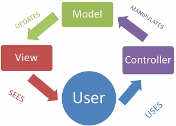
\includegraphics{mvc}
%\end{figure}

\bigskip
De models, views en controllers in het component zijn de volgende: \\

Voor de \textbf{agenda} sectie: \\

\begin{itemize}
\item items
\item itemform
\item item
\end{itemize}

Voor de \textbf{download} sectie: \\

\begin{itemize}
\item newsitems
\item newsitemform
\item newsitem
\end{itemize}

Voor de \textbf{medewerker nieuws} sectie: \\

\begin{itemize}
\item downloads
\item downloadform
\item download
\end{itemize}


Daarnaast is en een \textbf{portal} view toegevoegd.

\subsection{De logische opbouw van het component}

Het Joomla component bevat een \textbf{site} kan en een \textbf{administratie} kant. \\
De opbouw van het component bevat een \textbf{xml} file die de metadata van het component bijhoud. \\
Dat wil zeggen: \\
\begin{itemize}
\item De gegevens voor de auteur, omschrijving, maakdatum en dergelijke. \\
\item De gegevens voor de SQL interactie. (install en uninstall scripts). Deze gaat over de achterliggende gegevens. (zie ook hoofdstuk gegevensanalyse)  \\
\item De gegevens voor de \textbf{language files}. Deze leggen een vertaalslag voor verschillende labels in het component, zodat deze zowel in het engels, als in het nederlands beschikbaar wordt.
\item De gegevens voor de MVC (Model-View-Controller) interface.\\
\item De gegevens voor de \textbf{table classes} die de database interactie regelen. \\
\end{itemize}

Deze \textbf{xml} file regelt dus, op het moment dat de zipfile aan Joomla wordt aangeboden, hoe de installatie ervan zich dient te votrekken. \\

\newpage
\section{gegevensananalyse en ontwerp}

De achterliggende database bestaat uit vier tabellen. \\
\begin{itemize}
\item \#\_\_tks\_agenda\_download \\
\item \#\_\_tks\_agenda\_newsitems \\
\item \#\_\_tks\_agenda\_items \\
\item \#\_\_tks\_agenda\_recurring \\
\end{itemize}
Waarvan de laatste twee en relatie hebben met elkaar. \\

Joomla vervangt de prefix \textbf{\#\_\textunderscore} door de gegeven prefix van de 
namen van de Joomla tabellen, die bij installatie worden gegenereerd. \\

Het entiteiten relatie diagram is dan ook eenvoudig: \\

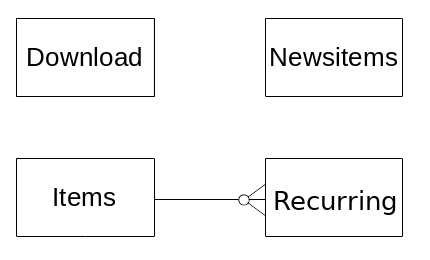
\includegraphics{erd}

Waar de \textbf{items} tabel en de \textbf{recurring} tabel een relatie hebben met elkaar. \\
Dit is alles wat er nodig is om de metadata van het component op te slaan. \\

\newpage
\section{functioneel ontwerp}

Bij het schrijven van het functioneel ontwerp houd ik me niet aan enige standaard of (klassieke) ontwikkelingsmethodologie\"{e}n. Dit niet alleen omdat het een reconstructie betreft van een bestaand produkt, waarbij dit ontwerp niet geleverd is, ook omdat het een eenvoudige opdracht betreft. Wel heb ik de overweging, dat mocht het geval zijn dat Takties mij vraagt componenten te maken, mij wel aan eenduidige richtlijnen te houden. \\
(In zulks een geval zou ik een template schrijven voor zowel een component als de documentatie ervan, maar dit is vooralsnog niet aan de orde). \\

Ik zou bij functioneel ontwerp kunnen denken aan: \\

\begin{itemize}
\item UML, met uitgebreide use-cases en alle andere relevante schema's.
\item System Development Methodology, oud maar bruikbaar. (daarnaast ben ik er goed in onderlegd).
\item Scrum, Rapid Application Development en soortgelijke.
\end{itemize}

Een grote vraag die ik me daarbij kan stellen is "Welke techniek past het beste in de organisatie, en bij het product?" \\

In dit project ga ik eigenlijk de omgekeerde richting als gewend is. \\
Ik maak aan de hand van het bestaande project een opsomming van de functionaliteiten, in plaats van omgekeerd. \\

Dit is nuttig voor analyse van het project, en verschaft inzicht over enventuele aanpassingen. \\


\textcolor{red}{\textbf{In deze versie van het document is de opsomming van functionaliteiten nog niet beschikbaar.}}
	
%De functies zijn: \\

%\begin{itemize}
%\item TODO \\
%\end{itemize}

\newpage
\subsection{Klassenhierarchie}

Het component gebruikt verschillende klassen uit de API, die Joomla definieerd. \\

De onderstaande opsomming reflecteerd de klassenhierarchie. De klassen die Joomla definieerd beginnen met een hoofdletter J, de klassen die takties definieerd beginnen met tks.\\

\begin{itemize}
\item JComponentRouterBase
\begin{itemize}
	\item tks\_agendaRouter
\end{itemize}
\item JControllerForm
\begin{itemize}
	\item tks\_agendaControllerNewsitemForm
	\item tks\_agendaControllerDownloadForm
\end{itemize}
\item JControllerLegacy
\begin{itemize}
	\item tks\_agendaController 
	\item tks\_agendaControllerNewsitem 
	\item tks\_agendaControllerDownload 
	\item tks\_agendaControllerDownload 
\end{itemize}
\item JModelForm
\begin{itemize}
	\item tks\_agendaModelNewsitemForm
	\item tks\_agendaModelItemForm  
	\item tks\_agendaModelDownloadForm
\end{itemize}
\item JModelItem
\begin{itemize}
	\item tks\_agendaModelItem
	\item tks\_agendaModelDownload
	\item tks\_agendaModelNewsitem
\end{itemize}
\item JModelList
\begin{itemize}
	\item tks\_agendaModelItems
	\item tks\_agendaModelDownloads
	\item tks\_agendaModelNewsitems
\end{itemize}
\end{itemize}
\newpage
\begin{itemize}
\item JTable
\begin{itemize}
	\item tks\_agendaTableitem  
	\item tks\_agendaTablenewsitem  
	\item tks\_agendaTabledownload 
\end{itemize}
\item JViewLegacy
\begin{itemize}
	\item tks\_agendaViewDownloadform
	\item tks\_agendaViewitems
	\item tks\_agendaViewitems
	\item tks\_agendaViewNewsitems
	\item tks\_agendaViewNewsitem
	\item tks\_agendaViewItem 
	\item tks\_agendaViewItem
	\item tks\_agendaViewDownload
	\item tks\_agendaViewPortal  
	\item tks\_agendaViewItemform
	\item tks\_agendaViewDownloads
	\item tks\_agendaViewNewsitemform
	\item tks\_agendaViewtks\_agenda
\end{itemize}
\item tks\_agendaController
\begin{itemize}
	\item tks\_agendaControllerItem  
	\item tks\_agendaControllerItems 
	\item tks\_agendaControllerDownloads 
	\item tks\_agendaControllerItemForm
	\item tks\_agendaControllerNewsitems 
\end{itemize}
\end{itemize}

Merk op dat all klassen die hier opgesomd staan een extensie zijn van Joomla gedefinieerde klassen, op \textbf{tks\_agendaController} na. \\
De klassen die geen extensie zijn van andere klassen de volgende: \\

\begin{itemize}
\item tks\_agendaHelper    
\item tks\_agendaSiteFrontendHelper    
\end{itemize}

De hierarchie een laag hierboven teken ik niet, omdat dit Joomla API specifieke klassen zijn. Raadpleeg de Joomla API documentatie voor de details. \\

\newpage
\subsection{Klassendiagram}

\textcolor{red}{\textbf{In deze versie van het document is het klassendiagram nog niet beschikbaar.}}

\subsection{Dialoogstructuur}

\textcolor{red}{\textbf{In deze versie van het document is de weergave van de dialoogstructuur nog niet beschikbaar.}}

\newpage
\section{technisch ontwerp}

Het technisch ontwerp bestaat uit de \textbf{phpdoc} gegenereerde API reference. \\
Deze is in site formaat en is gepubliceerd op de testomgeving.

\newpage
\section{implementatie en testen}

Bij het implementeren en testen dien ik testcases op te tekenen die de functionaliteiten uit het functioneel ontwerp proberen om zo eventuele fouten aan het licht te brengen.

\textcolor{red}{\textbf{Op moment van schrijven zijn de testcases nog niet beschikbaar}}

\section{status van het project}

Momenteel is het project dus nog in volle gang. Essentieel is het goed onder de loep nemen van de update functie van agenda items. \\
Wat het documenteren en testen betreft, wil ik met Takties in overleg treden over wat een einddocument (zoals deze) allemaal moet reflecteren. \\
Voor toekomstige projecten die Joomla componenten zijn, is het misschien goed een apart document te maken met eenduidige richtlijnen en werkwijzen.


\end{document}
